\documentclass{article} 

\usepackage[utf8]{inputenc} 

\usepackage[T1]{fontenc}
\usepackage{wrapfig}
\usepackage{graphicx}

\usepackage{subfig}

\title{Actividad 9}

\author{Ricardo Ruiz Hernández}

\date{30 de Abril, 2018}
 

\begin{document}

\maketitle 
\section*{Introducción}
La presente actividad nos presenta un sistema de álgebra computacional, el cual nos brinda la posibilidad de escribir cálculo, álgebra, e incluso preguntas estadísticas. Dicho sistema diseñado por el MIT en los 60's, se denomina WXMaxima. 

\section*{Aritmética}
Los valores se consideran como entrada, mientras que los resultados como salida; los primeros son representados por el símbolo de porcentaje, i, así como un número que dependerá del orden asignado.\\
Algunos de los símbolos utilizados son:
\begin{itemize}
\item Logaritmo natural: log(a)
\item Raíz enésima: (1/n)
\item Suma: +
\item Resta: -
\item Multiplicación: *


\section*{Derivación}
Para derivar directamente una función real de variable real podemos usar directamente la orden "diff". Esta orden actúa tanto con funciones como con expresiones.\\

\begin{center}
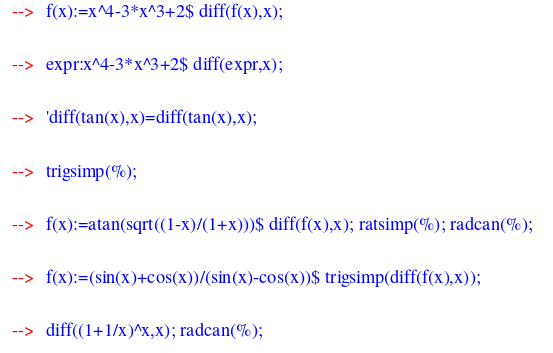
\includegraphics[scale=0.5]{Act92.png}
\end{center}

Si además queremos hallar el valor de la derivada en un punto concreto, basta combinar la orden "diff" con la orden "ev" (o con la orden "subst").

\begin{center}
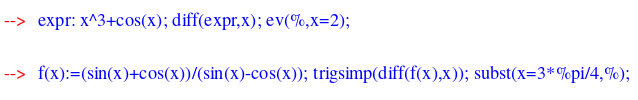
\includegraphics[scale=0.5]{Act93.png}
\end{center}

Es más recomendable definirla como función, para luego
evaluarla o representarla gráficamente como tal. Observemos que esto no debe hacerse como una definición directa, sino a través de la orden "define".

\begin{center}
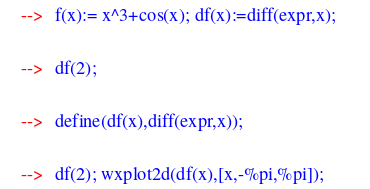
\includegraphics[scale=0.5]{Act94.png}
\end{center}
La orden "diff" también permite derivar funciones definidas implícitamente. Sin embargo, para ello habremos de combinar la instrucción "diff" con la orden "depends"
\begin{center}
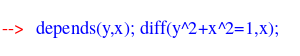
\includegraphics[scale=0.5]{Act95.png}
\end{center}

\section{Ejemplo}
\subsection*{Máximos y mínimos relativos}
Calculemos los extremos relativos de la función $f(x)=2x^{4}+4x$
\begin{center}
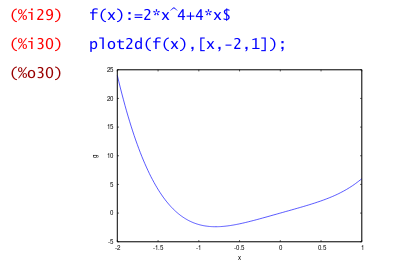
\includegraphics[scale=0.5]{Act96.png}
\end{center}

Parece que hay un mínimo en las proximidades de -1. Para confirmarlo, calculamos los puntos críticos de f.

\begin{center}
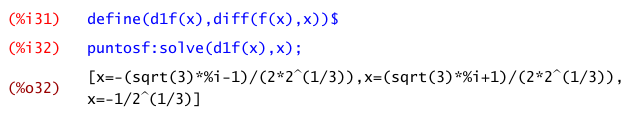
\includegraphics[scale=0.5]{Act97.png}
\end{center}

Observamos que hay sólo una raíz real que es la única que nos interesa.

\begin{center}
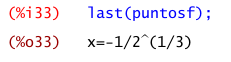
\includegraphics[scale=0.5]{Act98.png}
\end{center}

Llamamos a el único punto crítico que hemos obtenido, y evaluamos en él la segunda derivada:
\begin{center}
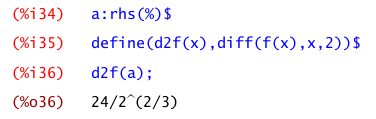
\includegraphics[scale=0.5]{Act99.png}
\end{center}
Por tanto la función f tiene un mínimo relativo en dicho punto a.


\section{Conclusiones}
Considero esta actividad una buena experiencia en el manejo de los CAS. Francamente, se me dificultó un poco al principio, pero una vez que entendí la interfaz, todo resultó más fluido. 

\section{Referencias}
\item $A. Maxima Tutorial. (2018). Def.fe.up.pt. 28 de Abril de 2018, https://def.fe.up.pt/dynamics/maxima_tutorial.html$
\item $wxMaxima Tutorials. (2018). Scotchildress.com. 28 de Abril de 2018, http://www.scotchildress.com/wxmaxima/$

\section{Apéndice}
\item ¿Cuál fue tú primera impresión de wxMáxima?
Me pareció interesante la interface y el nuevo lenguaje.
\item ¿Crees que esta herramienta puede ser útil en otros de tus cursos?
Si, porque es una herramienta que no es extensa y es práctica.
\item ¿Qué se te dificultó más en esta actividad?
Al principio, el lenguaje.
\item ¿Se te hizo compleja esta actividad? ¿Cómo la mejorarías? 
En términos generales no. No tengo nada que agregarle.

\end{itemize}
\end{document}
